\subsection{Package \lstinline!cryptocast.util!}
Utility classes that are not specific to CryptoCast and don't fit any of the other packages.

\noindent\begin{minipage}[t]{5cm}
\vspace{0.3em}
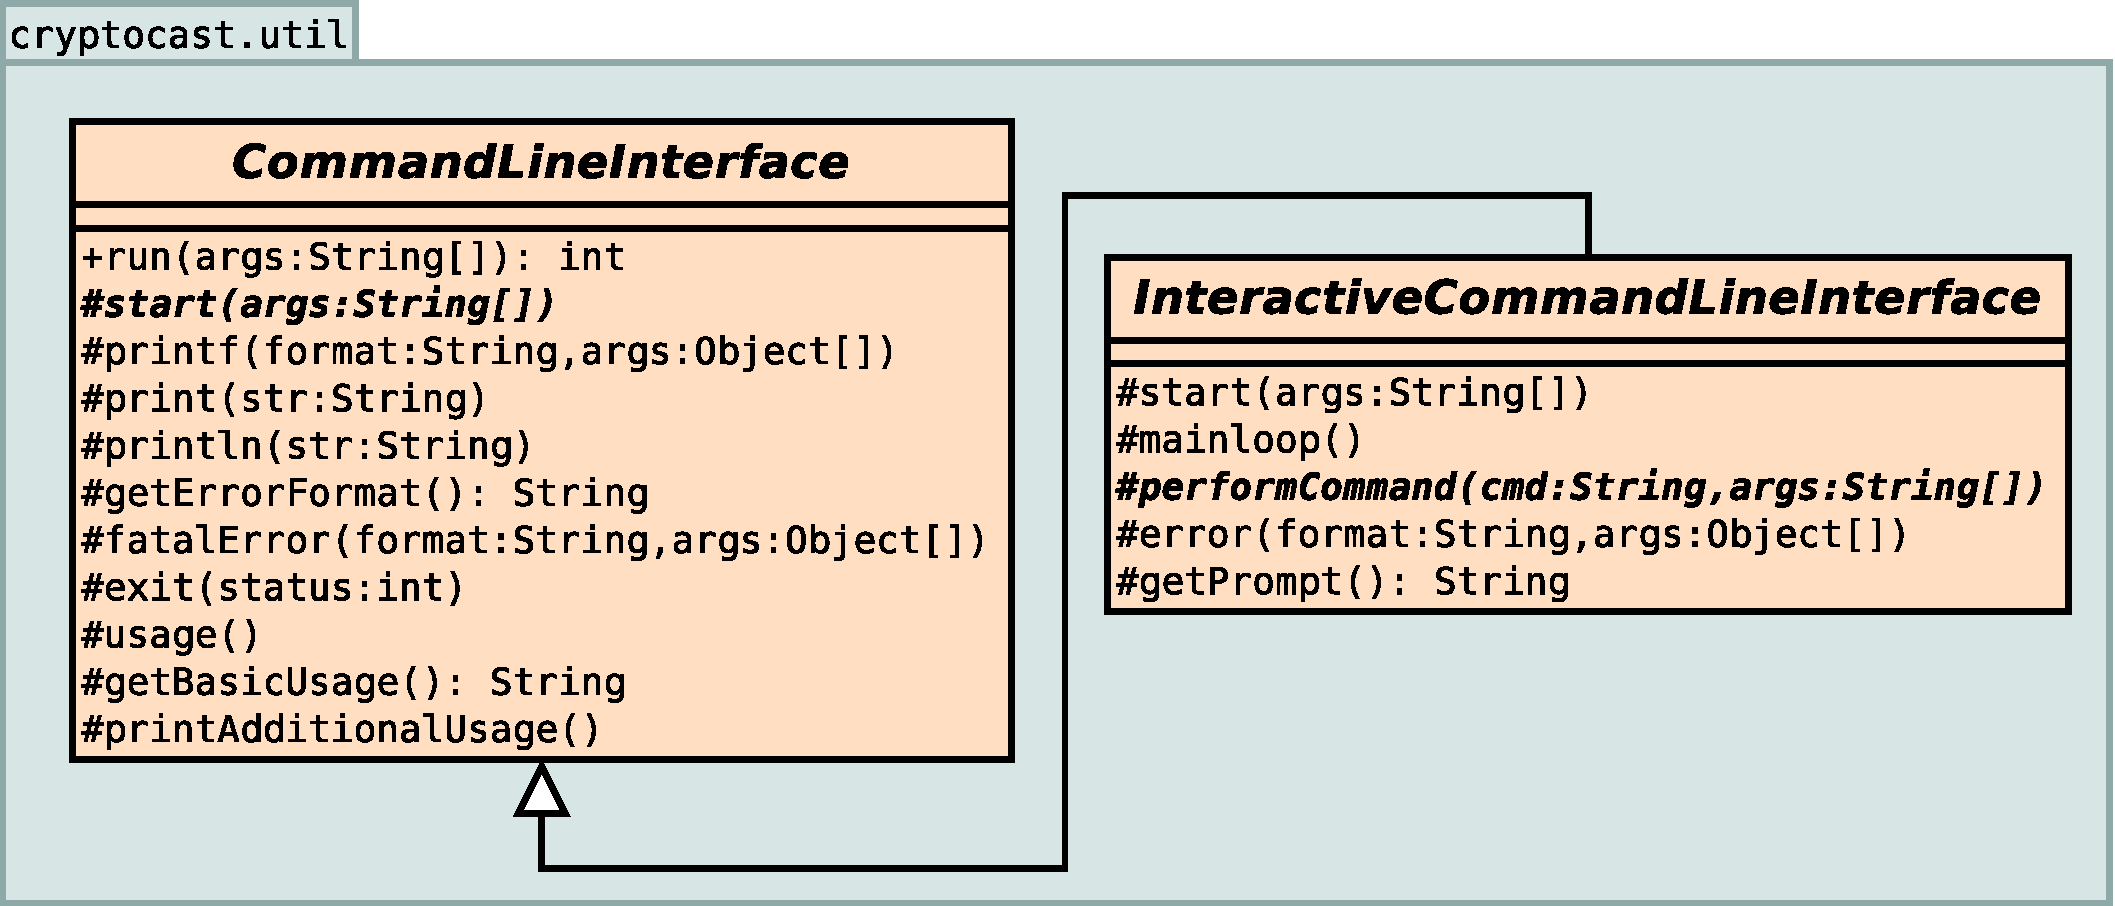
\includegraphics[width=300px]{class_diagrams/cryptocast_util.pdf}
\end{minipage}

\subsubsection{Class \lstinline|CommandLineInterface|}
A simple framework for command line programs. \\
\noindent\begin{minipage}[t]{5cm}
\vspace{0.3em}
\hspace*{2em}
\begin{tikzpicture}
\umlclass[type=abstract]{CommandLineInterface}{

}{
+ run(args : String[]) : int \\ \umlvirt{\# start(args : String[])} \\ \# printf(format : String, args : Object[]...) \\ \# print(str : String) \\ \# println(str : String) \\ \# getErrorFormat() : String \\ \# fatalError(format : String, args : Object[]...) \\ \# exit(status : int) \\ \# usage() \\ \# getBasicUsage() : String \\ \# printAdditionalUsage()
}
\end{tikzpicture}
\vspace{0.3em}
\end{minipage}




\textbf{\sffamily Constructors}
\begin{itemize}
\item \lstinline|public| \lstinline|CommandLineInterface|\lstinline|(InputStream in, PrintStream out, PrintStream err)|\\ \\[-0.6em]
Initializes a new CLI instance
\begin{itemize}
\item \lstinline|in|: The stream for program input
\item \lstinline|out|: The stream for program output
\item \lstinline|err|: The stream for error output
\end{itemize}



\end{itemize}


\textbf{\sffamily Methods}
\begin{itemize}
\item \lstinline|public int| \lstinline|run|\lstinline|(String[] args)|\\ \\[-0.6em]
Runs the application.
\begin{itemize}
\item \lstinline|args|: The command line arguments
\end{itemize}

\emph{Returns:} The exit code

\item \lstinline|protected abstract void| \lstinline|start|\lstinline|(String[] args)|\\ \\[-0.6em]
The main program logic (must be overridden by subclasses)
\begin{itemize}
\item \lstinline|args|: The command line arguments
\end{itemize}



\item \lstinline|protected void| \lstinline|printf|\lstinline|(String format, Object[] args...)|\\ \\[-0.6em]
Prints a string to the output stream
\begin{itemize}
\item \lstinline|format|: The string to print (printf format string)
\item \lstinline|args|: The printf arguments
\end{itemize}



\item \lstinline|protected void| \lstinline|print|\lstinline|(String str)|\\ \\[-0.6em]
Prints a string to the output stream
\begin{itemize}
\item \lstinline|str|: The string to print
\end{itemize}



\item \lstinline|protected void| \lstinline|println|\lstinline|(String str)|\\ \\[-0.6em]
Prints a string to the output stream after appending a newline
\begin{itemize}
\item \lstinline|str|: The string to print
\end{itemize}



\item \lstinline|protected String| \lstinline|getErrorFormat|\lstinline|()|\\ \\[-0.6em]
\emph{Returns:} the string format to use for writing error messages to the
 screen.



\item \lstinline|protected void| \lstinline|fatalError|\lstinline|(String format, Object[] args...)|\\ \\[-0.6em]
Prints an error and exits
\begin{itemize}
\item \lstinline|format|: The error message (printf format string)
\item \lstinline|args|: The printf arguments
\end{itemize}



\item \lstinline|protected void| \lstinline|exit|\lstinline|(int status)|\\ \\[-0.6em]
Exits the application
\begin{itemize}
\item \lstinline|status|: The exit code
\end{itemize}



\item \lstinline|protected void| \lstinline|usage|\lstinline|()|\\ \\[-0.6em]
Prints usage information



\item \lstinline|protected String| \lstinline|getBasicUsage|\lstinline|()|\\ \\[-0.6em]
\emph{Returns:} basic usage information for the program (should be overridden)



\item \lstinline|protected void| \lstinline|printAdditionalUsage|\lstinline|()|\\ \\[-0.6em]
Prints additional usage information (may be overridden)



\end{itemize}

\subsubsection{Class \lstinline|CommandLineInterface.Exit|}
Signals the exit of the application. \\
\noindent\begin{minipage}[t]{5cm}
\vspace{0.3em}
\hspace*{2em}
\begin{tikzpicture}
\umlclass[]{CommandLineInterface.Exit}{

}{
+ getStatus() : int
}
\end{tikzpicture}
\vspace{0.3em}
\end{minipage}



\textbf{\sffamily Superclasses and Interfaces}
\begin{itemize}
\item \lstinline|java.lang.Throwable|
\end{itemize}


\textbf{\sffamily Constructors}
\begin{itemize}
\item \lstinline|public| \lstinline|CommandLineInterface.Exit|\lstinline|(int status)|\\ \\[-0.6em]
Initializes a new Exit instance
\begin{itemize}
\item \lstinline|status|: The exit code
\end{itemize}



\end{itemize}


\textbf{\sffamily Methods}
\begin{itemize}
\item \lstinline|public int| \lstinline|getStatus|\lstinline|()|\\ \\[-0.6em]
\emph{Returns:} the exit code



\end{itemize}

\subsubsection{Class \lstinline|InteractiveCommandLineInterface|}
A framework class to implement interactive command-line interfaces. The class implements
 a read-parse-execute main loop and provides hooks for subclasses to implement the missing
 functionality. \\
\noindent\begin{minipage}[t]{5cm}
\vspace{0.3em}
\hspace*{2em}
\begin{tikzpicture}
\umlclass[type=abstract]{InteractiveCommandLineInterface}{

}{
\# start(args : String[]) \\ \# mainloop() \\ \umlvirt{\# performCommand(cmd : String, args : String[])} \\ \# error(format : String, args : Object[]...) \\ \# getPrompt() : String
}
\end{tikzpicture}
\vspace{0.3em}
\end{minipage}



\textbf{\sffamily Superclasses and Interfaces}
\begin{itemize}
\item \lstinline|cryptocast.util.CommandLineInterface|
\end{itemize}


\textbf{\sffamily Constructors}
\begin{itemize}
\item \lstinline|public| \lstinline|InteractiveCommandLineInterface|\lstinline|(InputStream in, PrintStream out, PrintStream err)|\\ \\[-0.6em]
Initializes a new interactive CLI instance
\begin{itemize}
\item \lstinline|in|: The stream for program input
\item \lstinline|out|: The stream for program output
\item \lstinline|err|: The stream for error output
\end{itemize}



\end{itemize}


\textbf{\sffamily Methods}
\begin{itemize}
\item \lstinline|protected void| \lstinline|start|\lstinline|(String[] args)|\\ \\[-0.6em]
The main program logic. This method just starts the main loop.
\begin{itemize}
\item \lstinline|args|: The command line arguments (ignored by default)
\end{itemize}



\item \lstinline|protected void| \lstinline|mainloop|\lstinline|()|\\ \\[-0.6em]
Starts the interactive Prompt-Read-Evaluate main loop.



\item \lstinline|protected abstract void| \lstinline|performCommand|\lstinline|(String cmd, String[] args)|\\ \\[-0.6em]
Executes the given command with the given arguments. Must be implemented by subclasses.
\begin{itemize}
\item \lstinline|cmd|: The command name
\item \lstinline|args|: The command arguments
\end{itemize}



\item \lstinline|protected void| \lstinline|error|\lstinline|(String format, Object[] args...)|\\ \\[-0.6em]
Helper function to trigger an error withing a command's execution and break out to
 the main loop.
\begin{itemize}
\item \lstinline|format|: The format string
\item \lstinline|args|: The format string arguments
\end{itemize}



\item \lstinline|protected String| \lstinline|getPrompt|\lstinline|()|\\ \\[-0.6em]
\emph{Returns:} The input prompt



\end{itemize}

\subsubsection{Class \lstinline|InteractiveCommandLineInterface.CommandError|}
An error within one of the commands. Will be caught by the main loop \\
\noindent\begin{minipage}[t]{5cm}
\vspace{0.3em}
\hspace*{2em}
\begin{tikzpicture}
\umlclass[]{InteractiveCommandLineInterface.CommandError}{

}{
+ getMessage() : String
}
\end{tikzpicture}
\vspace{0.3em}
\end{minipage}



\textbf{\sffamily Superclasses and Interfaces}
\begin{itemize}
\item \lstinline|java.lang.Throwable|
\end{itemize}


\textbf{\sffamily Constructors}
\begin{itemize}
\item \lstinline|public| \lstinline|InteractiveCommandLineInterface.CommandError|\lstinline|(String msg)|\\ \\[-0.6em]
Initializes the error
\begin{itemize}
\item \lstinline|msg|: The error message
\end{itemize}



\end{itemize}


\textbf{\sffamily Methods}
\begin{itemize}
\item \lstinline|public String| \lstinline|getMessage|\lstinline|()|\\ \\[-0.6em]
\emph{Returns:} The associated error message



\end{itemize}


